\documentclass{../source/zjureport}

\major{信息工程}
\name{箫宇 }
\title{实验设计报告}
\stuid{ }
\college{信息与电子工程学院}
\date{\today}
\lab{教4-421}
\course{数字信号处理}
\instructor{徐元欣}
\grades{}
\expname{确定性信号谱分析}
\exptype{验证}
\partner{--}

\begin{document}
    \makeheader
    \section{实验目的和要求}
    谱分析即求信号的频谱。本实验采用DFT/FFT技术对周期性信号进行谱分析。通过实验,
    了解用$X(k)$近似地表示频谱$X(e^{j\omega})$带来的栅栏效应、混叠现象和频谱泄漏,了解如何正
    确地选择参数(抽样间隔T、抽样点数N)。

    \section{实验内容和步骤}
        \subsection{选用最简单的周期信号:单频正弦信号、频率f=50赫兹,进行谱分析。}
        \subsection{谱分析参数可以从下表中任选一组(也可自定)。对各组参数时的序列,
        计算:一个正弦周期是否对应整数个抽样间隔?观察区间是否对应整数个正弦周期?}

        \begin{table}[H]
            \centering
            \begin{tabular}{|c|c|c|c|}
            \hline
            \multicolumn{1}{|l|}{\textbf{信号频率f(赫兹)}} & \multicolumn{1}{l|}{\textbf{谱分析参数}} & \multicolumn{1}{l|}{\textbf{抽样间隔T(s)}} & \multicolumn{1}{l|}{\textbf{截断长度N}} \\ \hline
            50                                       & 第一组参数                               & 0.000625                               & 32                                  \\ \hline
            50                                       & 第二组参数                               & 0.005                                  & 32                                  \\ \hline
            50                                       & 第三组参数                               & 0.0046875                              & 32                                  \\ \hline
            50                                       & 第四组参数                               & 0.004                                  & 32                                  \\ \hline
            50                                       & 第五组参数                               & 0.0025                                 & 16                                  \\ \hline
            \end{tabular}
            \end{table}

        \subsection{对以上几个正弦序列,依次进行以下过程。}
            \subsubsection{观察并记录一个正弦序列的图形(时域)、频谱(幅度谱、频谱实部、频谱虚部)形状、幅度谱的第一个峰的坐标(U,V)。}
            \subsubsection{分析抽样间隔T、截断长度N(抽样个数)对谱分析结果的影响;}
            \subsubsection{思考$X(k)$与$X(e^{j\omega})$的关系;}
            \subsubsection{讨论用$X(k)$近似表示$X(e^{j\omega})$时的栅栏效应、混叠现象、频谱泄漏。}

    \section{主要仪器设备}
        MATLAB编程。

    \section{操作方法和实验步骤}
        (参见“二、实验内容和步骤”)
    
    \section{实验数据记录和处理}
        \lstinputlisting[caption = 主函数 , language = matlab]{code/Problem2.m}
        \newpage
        \lstinputlisting[caption = 绘图函数 , language = matlab]{code/drawPic.m}

    \section{实验结果与分析}
        \subsection{序列图像}
            \begin{figure}[H]
                \centering
                \begin{minipage}[t]{0.48\textwidth}
                \centering
                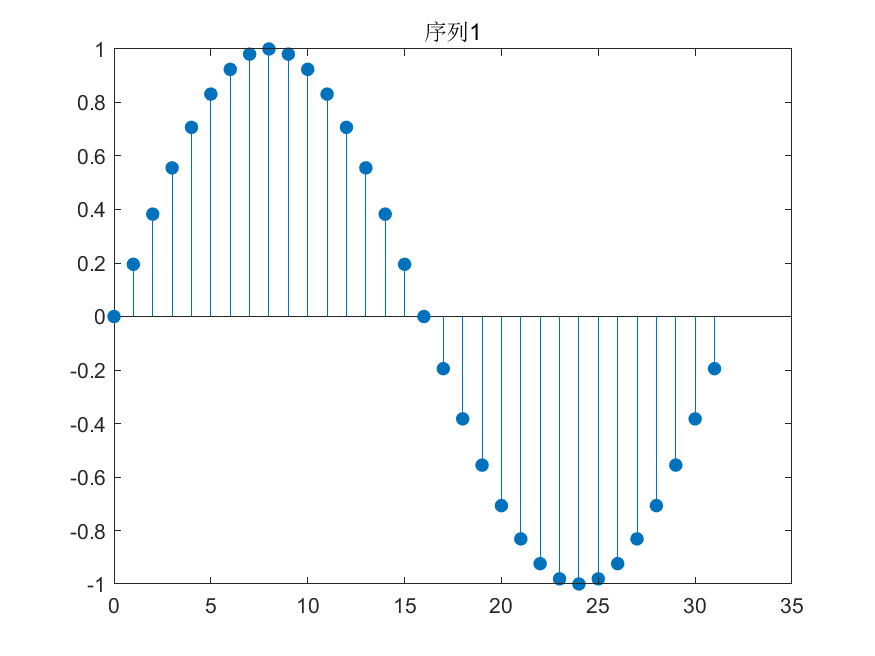
\includegraphics[width=\textwidth]{figure/序列1.png}
                \end{minipage}
                \begin{minipage}[t]{0.48\textwidth}
                \centering
                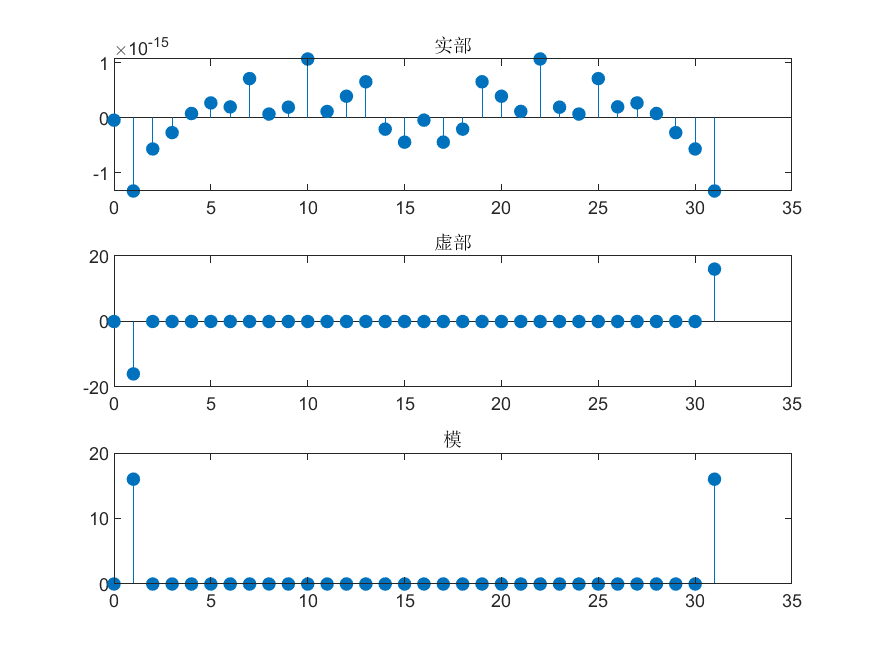
\includegraphics[width=\textwidth]{figure/频谱_序列1.png}
                \end{minipage}
                \caption{序列一及其频谱}
            \end{figure}

            \begin{figure}[H]
                \centering
                \begin{minipage}[t]{0.48\textwidth}
                \centering
                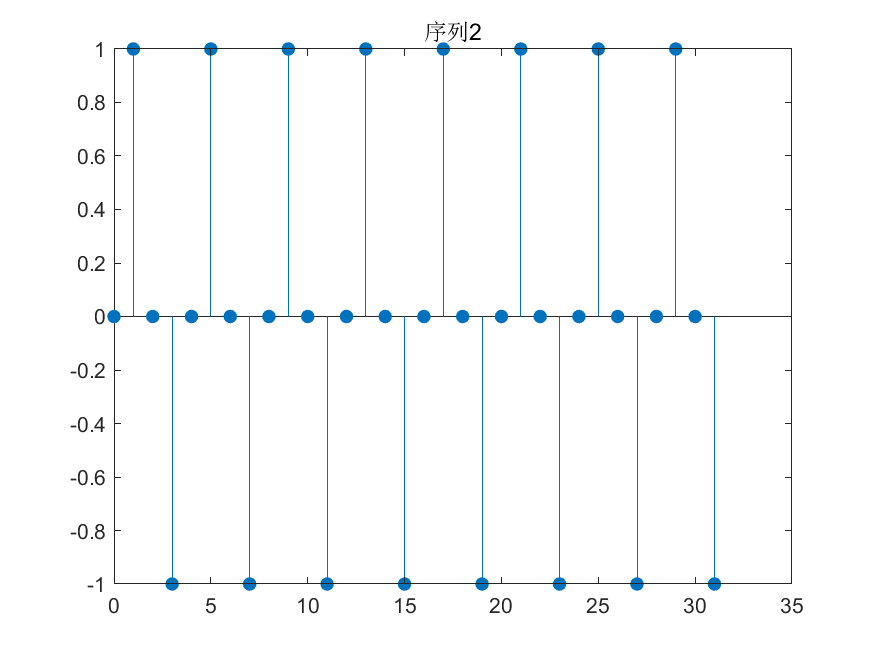
\includegraphics[width=\textwidth]{figure/序列2.png}
                \end{minipage}
                \begin{minipage}[t]{0.48\textwidth}
                \centering
                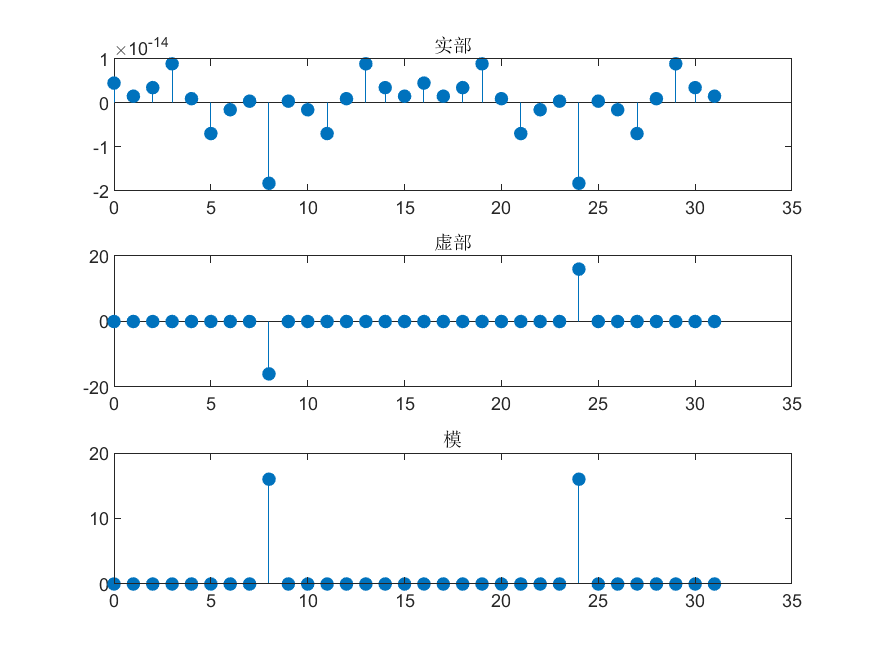
\includegraphics[width=\textwidth]{figure/频谱_序列2.png}
                \end{minipage}
                \caption{序列二及其频谱}
            \end{figure}

            \begin{figure}[H]
                \centering
                \begin{minipage}[t]{0.48\textwidth}
                \centering
                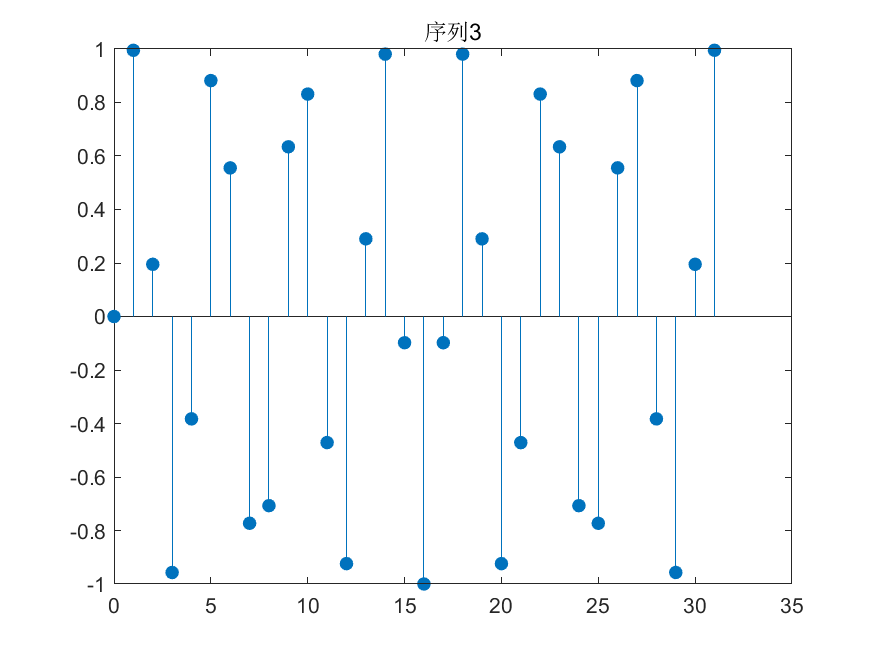
\includegraphics[width=\textwidth]{figure/序列3.png}
                \end{minipage}
                \begin{minipage}[t]{0.48\textwidth}
                \centering
                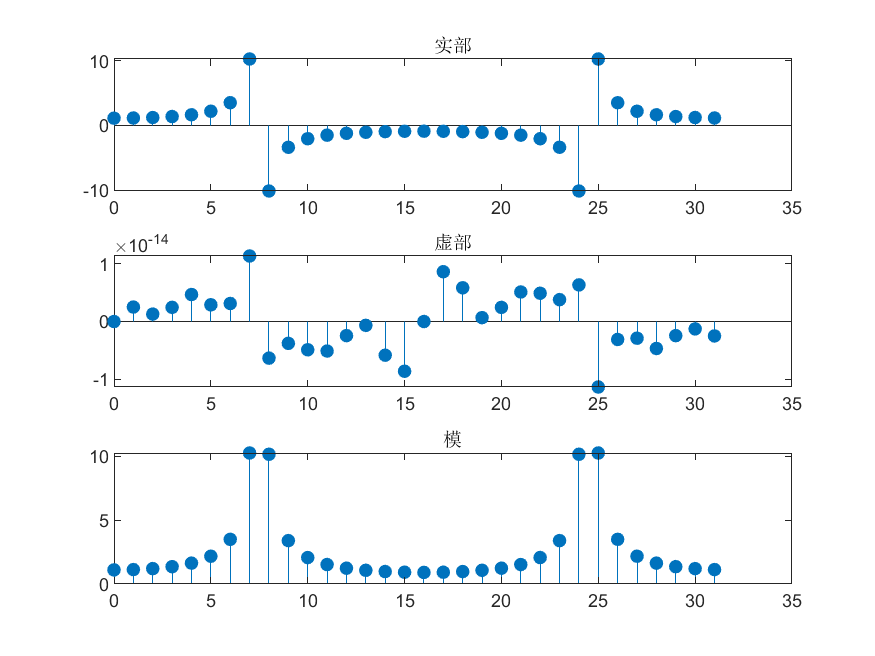
\includegraphics[width=\textwidth]{figure/频谱_序列3.png}
                \end{minipage}
                \caption{序列三及其频谱}
            \end{figure}

            \begin{figure}[H]
                \centering
                \begin{minipage}[t]{0.48\textwidth}
                \centering
                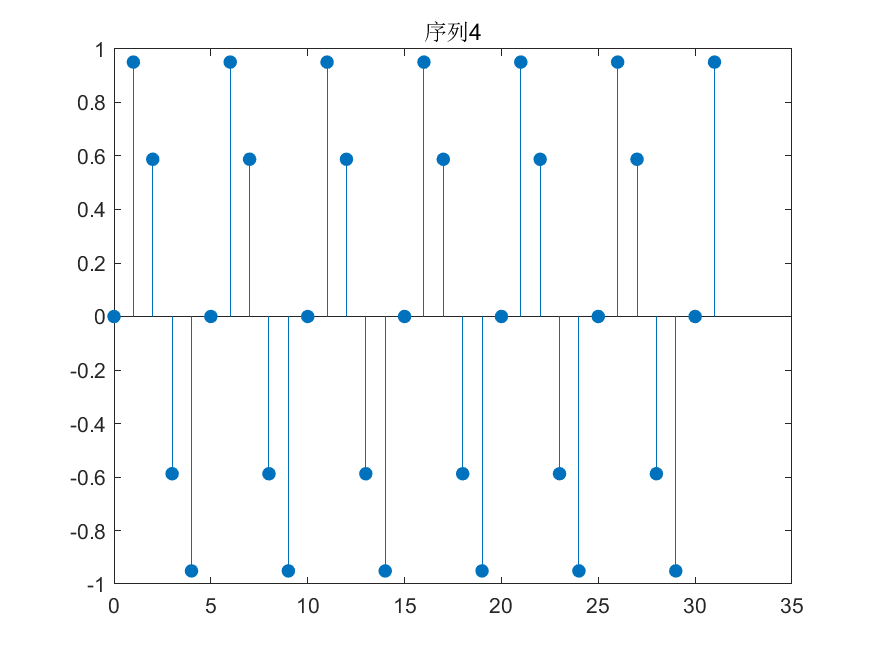
\includegraphics[width=\textwidth]{figure/序列4.png}
                \end{minipage}
                \begin{minipage}[t]{0.48\textwidth}
                \centering
                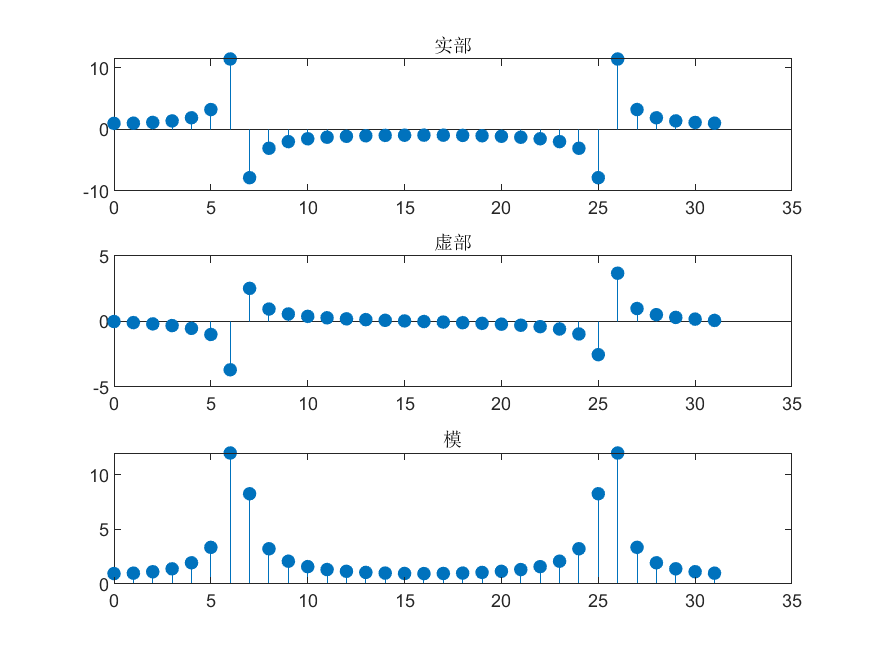
\includegraphics[width=\textwidth]{figure/频谱_序列4.png}
                \end{minipage}
                \caption{序列四及其频谱}
            \end{figure}

            \begin{figure}[H]
                \centering
                \begin{minipage}[t]{0.48\textwidth}
                \centering
                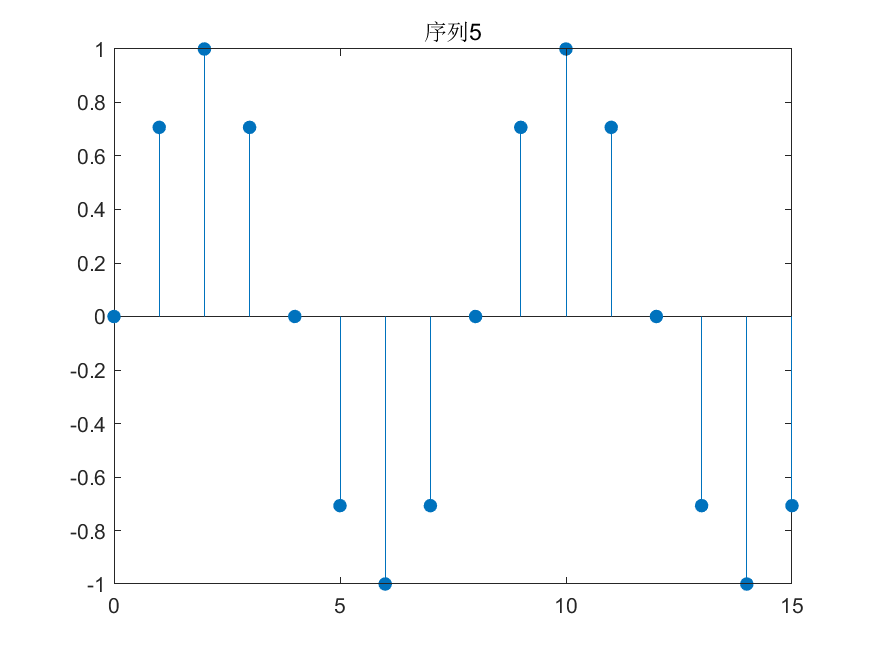
\includegraphics[width=\textwidth]{figure/序列5.png}
                \end{minipage}
                \begin{minipage}[t]{0.48\textwidth}
                \centering
                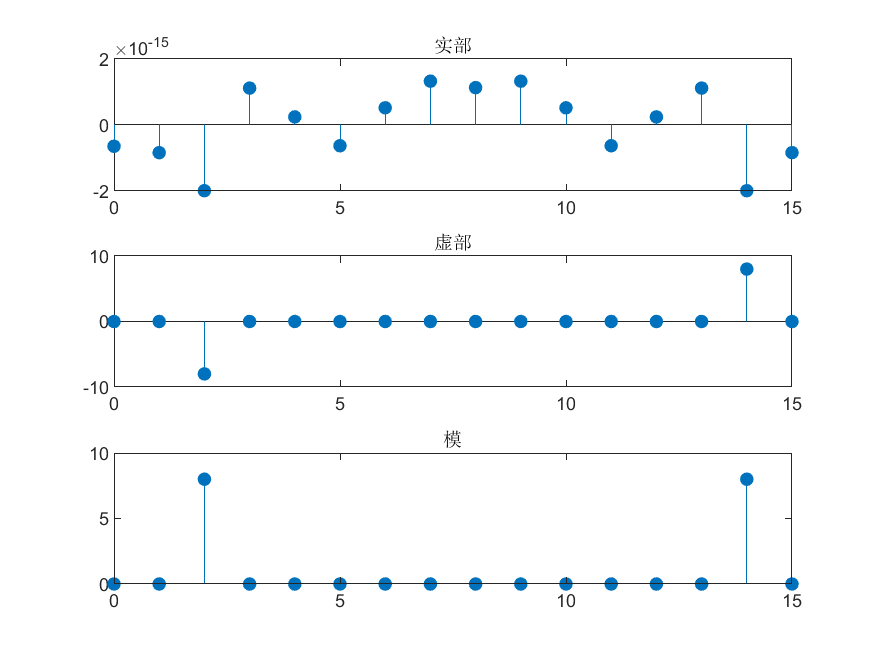
\includegraphics[width=\textwidth]{figure/频谱_序列5.png}
                \end{minipage}
                \caption{序列五及其频谱}
            \end{figure}

        \subsection{实验前预习有关概念,并根据上列参数来推测相应频谱的形状、谱峰所在频率(U)和谱峰的数值(V)、混叠现象和频谱泄漏的有无。}
        \begin{table}[H]
            \begin{tabular}{|c|c|c|c|c|c|c|}
            \hline
            \textbf{序列} & \textbf{一个周期为多少个抽样间隔} & \textbf{是否对应整数个正弦周期} & \textbf{U} & V     & 是否有混叠 & 是否有频谱泄露 \\ \hline
            序列一         & 32                    & 1                    & 1          & 16    & 否     & 否       \\ \hline
            序列二         & 4                     & 8                    & 8          & 16    & 否     & 否       \\ \hline
            序列三         & 4.27                  & 7.5                  & 7.5        & 10.25 & 否     & 有       \\ \hline
            序列四         & 5                     & 6.4                  & 6.4        & 12    & 否     & 有       \\ \hline
            序列五         & 8                     & 2                    & 2          & 8     & 否     & 否       \\ \hline
            \end{tabular}
            \end{table}

        \subsection{分析抽样间隔T、截断长度N(抽样个数)对谱分析结果的影响}
            抽样间隔越小,在时域中就越能够反映出该序列真实的图像。只有当抽样频率大于该信号最大频率的两倍在频谱
            中才不会发生混叠,观察本次实验中采样得到的五个序列,可以发现五个序列均满足奈奎斯特采样率,均未发生混叠。


            同时抽样的时间长短决定是否发生频谱泄漏,同时当
            采样同步时,窗口宽度等于整数个信号周期,矩形框的过零点与离散频点正好对齐,没有泄露

        \subsection{思考$X(k)$与$X(e^{j\omega})$关系}
            $X(k)$是$X(e^{j\omega})$上的均匀采样。

        \subsection{讨论用$X(k)$近似表示$X(e^{j\omega})$时的栅栏效应、混叠现象、频谱泄漏。}
            \begin{enumerate}
                \item 栅栏效应:因为$X(k)$是$X(e^{j\omega})$上的均匀采样,所以一定会产生栅栏效应,采样点数越多,间隔越小,栅栏效应就越弱
                \item 混叠效应:当采样频率高于信号最高频率的两倍时,不会发生混叠现象
                \item 频谱泄露:窗口函数的宽度等于整数个信号周期时,不会发生频谱泄露
            \end{enumerate}
        
        \subsection{观察实验结果(数据及图形)的特征,做必要的记录。}
            \begin{enumerate}
                \item 采样点数的数目会影响频谱的高度
                \item 序列三与序列四出现了频谱泄露,序列一、二与五没有出现
                \item 序列一、二与五被取到了整数个信号周期
            \end{enumerate}

        \subsection{用基本理论、基本概念来解释各种现象}
            因为$X(k)$是$X(e^{j\omega})$在$0-2\pi$上的均匀采样,所以可以看出序列1,3,5取到峰值的地方可以归为$\frac{\pi}{16},\frac{\pi}{2},\frac{\pi}{4}$,
            这一现象与我们理论计算出来的值相等。

            因为序列一、三与五是没有发生频谱泄露,所以这三个序列的频谱仅在理论计算出的位置;而序列三与四窗函数的宽度并不是
            信号周期的整数倍,所以发生了频谱泄露。

\end{document}